\begin{frame}[fragile]
\frametitle{DoubleML Workflow: 0. Problem Formulation}
\begin{columns}
\begin{column}{0.3\textwidth}
\pdftooltip{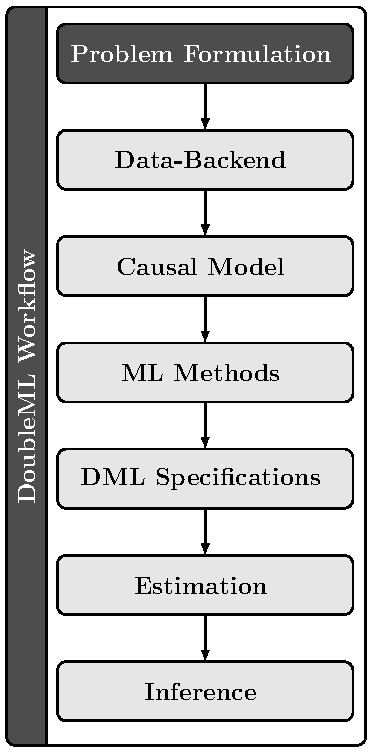
\includegraphics[width = \textwidth]{workflow/doubleml_workflow_problem.pdf}}{Description of Figure (alt-text): On the left hand side of the slide (and the following slides), there is a diagramm showing the seven steps of the DoubleML workflow. The fist step is the "Problem Formulation". The second step is the "Data-Backend". The third step is the "Causal Model". The fourth step is the choice of  "ML Methods". The fifth step is "DML Specifications". The sixth step is performing the "Estimation". The last step is then "Inference". In the following slides, each of the steps is explained in more detail. On each slide, the box of the corresponding workflow step is highlighted.}
\end{column}
\begin{column}{0.7\textwidth}
\textbf{Description of the Case Study and Data I}
\begin{itemize}
\small
\item 401(k) plans are pension accounts sponsored by employers
\item \textbf{Estimate the effect of 401(k) eligibility and participation on accumulated assets}
\item Problems: \textbf{Saver heterogeneity} and the fact that the \textbf{decision to enroll} in a 401(k) \textbf{is non-random}
\item \textbf{Conventional estimates} that do not account for saver heterogeneity and endogeneity of participation \textbf{will be biased}
\end{itemize}
\end{column}
\end{columns}
\end{frame}

\begin{frame}[fragile]
\frametitle{DoubleML Workflow: 0. Problem Formulation}
\begin{columns}
\begin{column}{0.3\textwidth}
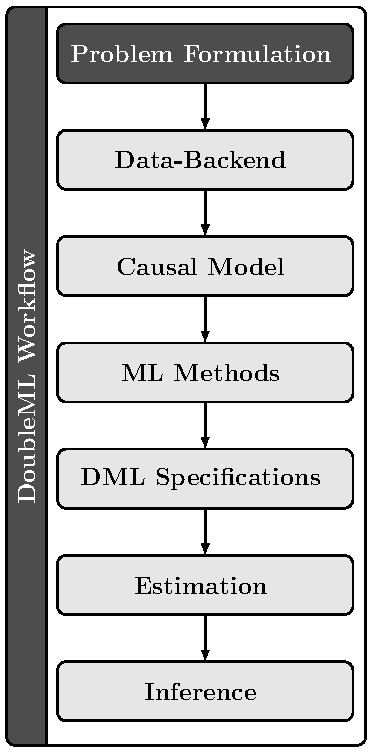
\includegraphics[width = \textwidth]{workflow/doubleml_workflow_problem.pdf}
\end{column}
\begin{column}{0.7\textwidth}
\textbf{Description of the Case Study and Data II}
\begin{itemize}
\small
\item \textbf{Eligibility} for enrolling in a 401(k) plan might be taken as \textbf{exogenous after conditioning} on a few observables of which the most important may be income
\item \textbf{The basic idea}:  Around the time 401(k)’s initially became available, people were unlikely to be basing their employment decisions on whether an employer offered a 401(k) but would instead focus on income and other aspects of the job
\item The data consist of 9,915 observations at the household level drawn from the 1991 Survey of Income and Program Participation (SIPP)
\item \textbf{Outcome variable: Net financial assets}
\end{itemize}
\end{column}
\end{columns}
\end{frame}

\begin{frame}[fragile]
\frametitle{DoubleML Workflow: 1. Data-Backend}
\begin{columns}
\begin{column}{0.3\textwidth}
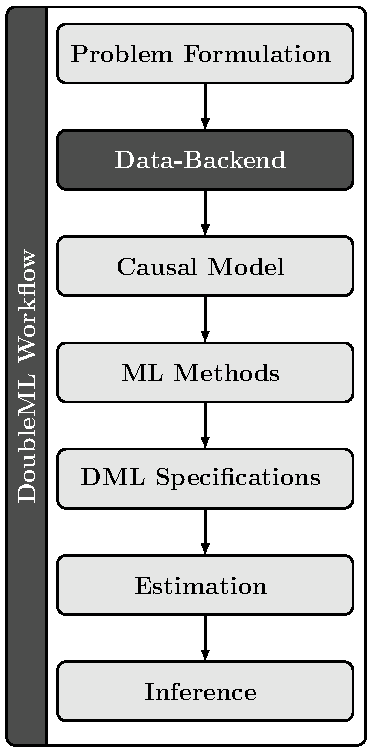
\includegraphics[width = \textwidth]{workflow/doubleml_workflow_data.pdf}
\end{column}
\begin{column}{0.7\textwidth}
\begin{itemize}
\item \textbf{DoubleMLData} from a data.table or data.frame
\end{itemize}
{\tiny
\begin{lstlisting}[language=Python,
backgroundcolor = \color{gray!20},
keywordstyle=\color{OliveGreen}, stringstyle=\color{BrickRed}]
library(DoubleML)
data = fetch_401k(return_type='data.table')
# Construct DoubleMLData object from data.table
dml_data = DoubleMLData$new(data, y_col='net_tfa', d_cols='e401',
	                    x_cols=c('age', 'inc', 'educ', 'fsize',
	                             'marr', 'twoearn', 'db', 'pira',
	                             'hown'))
	                        		 
data_frame = fetch_401k(return_type='data.frame')
# Construct DoubleMLData object from data.frame
dml_data_df = double_ml_data_from_data_frame(data_frame,
                                             y_col='net_tfa',
                                             d_cols='e401', 
                                             x_cols=c('age', 'inc',
                                                      'educ', 'fsize',
                                                      'marr', 'twoearn',
                                                      'db', 'pira',
                                                      'hown'))
\end{lstlisting}
}
\begin{itemize}
\item \textbf{DoubleMLData} from matrix
\end{itemize}
{\tiny
\begin{lstlisting}[language=Python,
backgroundcolor = \color{gray!20},
keywordstyle=\color{OliveGreen}, stringstyle=\color{BrickRed}]
# Simulate data
set.seed(3141); n_obs = 500; n_vars = 100; theta = 3; 
X = matrix(rnorm(n_obs*n_vars), nrow=n_obs, ncol=n_vars)
d = X[,1:3]%*%c(5,5,5) + rnorm(n_obs)
y = theta*d + X[, 1:3]%*%c(5,5,5) + rnorm(n_obs)

dml_data_sim =  double_ml_data_from_matrix(X, y, d)
\end{lstlisting}
}
\end{column}
\end{columns}
\end{frame}

\begin{frame}
\frametitle{DoubleML Workflow: 2. Causal Model}
\begin{columns}
\begin{column}{0.3\textwidth}
\pdftooltip{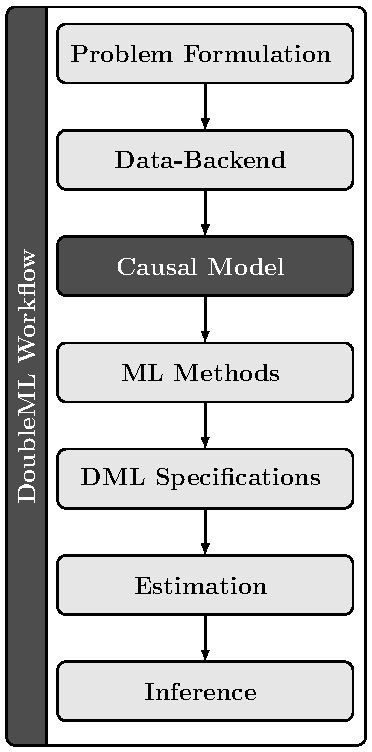
\includegraphics[width = \textwidth]{workflow/doubleml_workflow_causal.pdf}}{The figure shows a diagramm of the causal models that are currently implemented in DoubleML. On top, there is a box with annotation "DoubleML Models". From this box, two arrows go out into two boxes that are located on a layer below. In the box on the left hand side, it is written "partially linear treatment effect" with the formula for a partially linear regression model and an additive causal effect THETANULL associated with variable D. In the box on the right hand side, it is written "binary D and heterogeneous treatment effect" with a formula for a non-parameteric regression model. Each of the two boxes has an arrow going to a box with the question "Instrumental Variable?". If the answer to this question is yes, the arrows goes into the respective box that represents each of the causal models: The partially linear regression model without instrumental model called the "Partially linear regression (PLR) or the model with instrumental variable. The latter is called the "Partially linear IV regression (PLIV)". On the right hand side, the model without instrumental variable is called the "Interactive regression model (IRM)". The model with instrumental variable is called the "Interactive IV model (IIVM)".}
\end{column}
\begin{column}{0.7\textwidth}
\begin{itemize}
\item Specify a \textbf{causal model}
\end{itemize}
\vspace*{10pt}
\hspace*{-0.7cm}
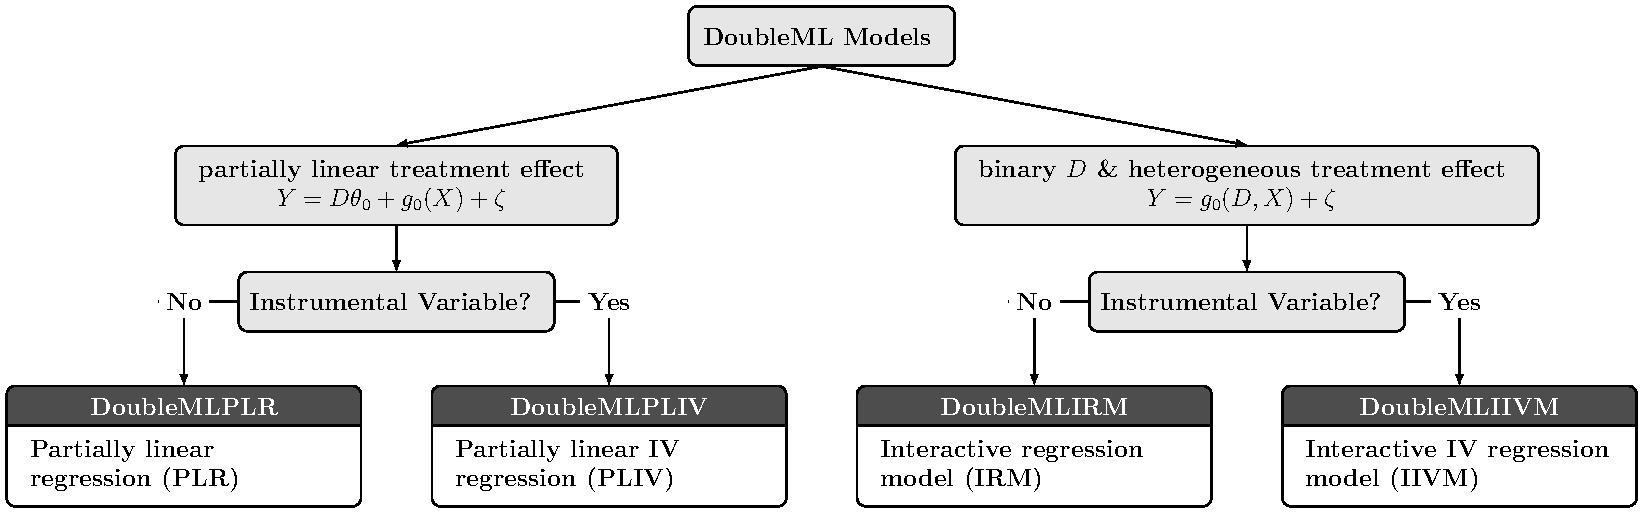
\includegraphics[width=1.17\textwidth]{workflow/doubleml_models.pdf}
\begin{itemize}
\item 401k data: Partially linear regression (PLR)
\end{itemize}
\vspace*{10pt}
\begin{center}
\pdftooltip{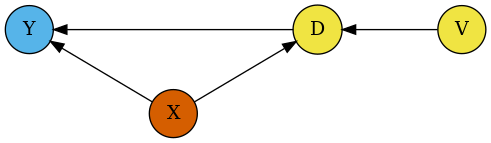
\includegraphics[width=0.8\textwidth]{pictures_and_logos/dag_plr2.png}}{A graph illustrating the  partially linear regression setting. There are four nodes in total: One for the dependent variable Y, one for the treatment variable D, one for the vector of confounding variables X and one for the stochastic error V. There are four directed edges in the figure, each illustrating a causal channel: From V into D, from D into Y, from X into Y and from X into D.}
\end{center}
\end{column}
\end{columns}
\end{frame}

\begin{frame}[fragile]
\frametitle{DoubleML Workflow: 3. ML Methods}
\begin{columns}
\begin{column}{0.3\textwidth}
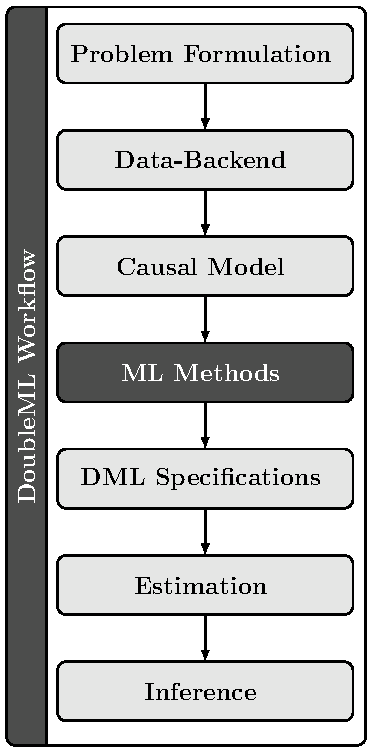
\includegraphics[width = \textwidth]{workflow/doubleml_workflow_ml.pdf}
\end{column}
\begin{column}{0.7\textwidth}
\begin{itemize}
\item Choose \textbf{ML methods} to approximate the nuisance functions
\item PLR
\begin{itemize}
\item $g_0(X) = \mathbb{E}(Y|X)$
\item $m_0(X) = \mathbb{E}(D|X)$
\end{itemize}
\item Random forest from ranger/mlr3learners.
\end{itemize}
{\tiny
\begin{lstlisting}[language=Python,
backgroundcolor = \color{gray!20},
keywordstyle=\color{OliveGreen}, stringstyle=\color{BrickRed}]
library(mlr3learners)
ml_g_rf = lrn("regr.ranger", max.depth = 7,
              mtry = 3, min.node.size = 3)
ml_m_rf = lrn("classif.ranger", max.depth = 5,
              mtry = 4, min.node.size = 7)
\end{lstlisting}
}
\begin{itemize}
\item Boosted trees from xgboost/mlr3extralearners
\end{itemize}
{\tiny
\begin{lstlisting}[language=Python,
backgroundcolor = \color{gray!20},
keywordstyle=\color{OliveGreen}, stringstyle=\color{BrickRed}]
ml_g_xgb = lrn("regr.xgboost",
               objective = "reg:squarederror",
               eta = 0.1, nrounds = 35)
ml_m_xgb = lrn("classif.xgboost",
               objective = "binary:logistic",
               eval_metric = "logloss",
               eta = 0.1, nrounds = 34)
\end{lstlisting}
}
\end{column}
\end{columns}
\end{frame}

\begin{frame}[fragile]
\frametitle{DoubleML Workflow: 4. DML Specifications}
\begin{columns}
\begin{column}{0.3\textwidth}
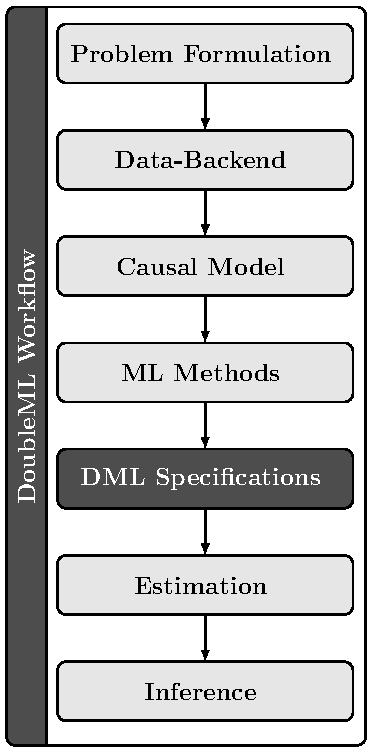
\includegraphics[width = \textwidth]{workflow/doubleml_workflow_dml.pdf}
\end{column}
\begin{column}{0.7\textwidth}
\begin{itemize}
\item \textbf{Initialize a DoubleMLPLR model}
\end{itemize}
{\tiny
\begin{lstlisting}[language=Python,
backgroundcolor = \color{gray!20},
keywordstyle=\color{OliveGreen}, stringstyle=\color{BrickRed}]
set.seed(123)
dml_plr_forest = DoubleMLPLR$new(dml_data,
                                 ml_g = ml_g_rf,
                                 ml_m = ml_m_rf,
                                 n_folds = 3)
\end{lstlisting}
}
\begin{itemize}
\item \textbf{Parametrize DoubleML models}
\begin{itemize}
\item \textbf{Resampling} (repeated cross-fitting): Number of repetitions \& folds
\item \textbf{DML algorithm}: dml1 vs.\ dml2
\item Neyman orthogonal \textbf{score function} (for PLR 'partialling out' or 'IV-type')
\end{itemize}
\end{itemize}
{\tiny
\begin{lstlisting}[language=Python,
backgroundcolor = \color{gray!20},
keywordstyle=\color{OliveGreen}, stringstyle=\color{BrickRed}]
set.seed(123)
dml_plr_forest = DoubleMLPLR$new(dml_data, ml_g = ml_g_rf,
                                 ml_m = ml_m_rf, n_folds=3, n_rep=1,
                                 score='partialling out',
                                 dml_procedure='dml2')
\end{lstlisting}
}
\end{column}
\end{columns}
\end{frame}

\begin{frame}[fragile]
\frametitle{DoubleML Workflow: 5. Estimation}
\begin{columns}
\begin{column}{0.3\textwidth}
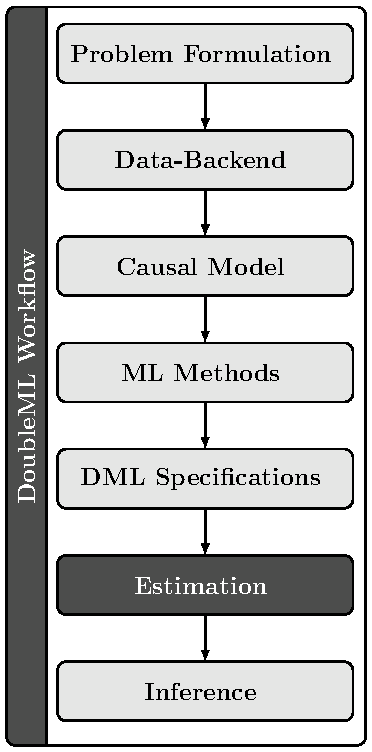
\includegraphics[width = \textwidth]{workflow/doubleml_workflow_est.pdf}
\end{column}
\begin{column}{0.7\textwidth}
\begin{itemize}
\item \textbf{Estimation} of the DoubleML model
\end{itemize}
{\tiny
\begin{lstlisting}[language=Python,
backgroundcolor = \color{gray!20},
keywordstyle=\color{OliveGreen}, stringstyle=\color{BrickRed}]
dml_plr_forest$fit()
\end{lstlisting}
}
\begin{itemize}
\item Estimated causal effect
\end{itemize}
{\tiny
\begin{lstlisting}[language=Python,
backgroundcolor = \color{gray!20},
keywordstyle=\color{OliveGreen}, stringstyle=\color{BrickRed}]
dml_plr_forest$coef
    e401 
8968.788
\end{lstlisting}
}
\begin{itemize}
\item Estimated standard error
\end{itemize}
{\tiny
\begin{lstlisting}[language=Python,
backgroundcolor = \color{gray!20},
keywordstyle=\color{OliveGreen}, stringstyle=\color{BrickRed}]
dml_plr_forest$se
    e401 
1341.061 
\end{lstlisting}
}
\begin{itemize}
\item \textbf{Summary} of the estimated effect
\end{itemize}
{\tiny
\begin{lstlisting}[language=Python,
backgroundcolor = \color{gray!20},
keywordstyle=\color{OliveGreen}, stringstyle=\color{BrickRed}]
dml_plr_forest$summary()
[1] "Estimates and significance testing of the effect of target variables"
     Estimate. Std. Error t value Pr(>|t|)    
e401      8969       1341   6.688 2.27e-11 ***
---
Signif. codes:  0 '***' 0.001 '**' 0.01 '*' 0.05 '.' 0.1 ' ' 1
\end{lstlisting}
}
\end{column}
\end{columns}
\end{frame}

\begin{frame}[fragile]
\frametitle{DoubleML Workflow: 6. Inference}
\begin{columns}
\begin{column}{0.3\textwidth}
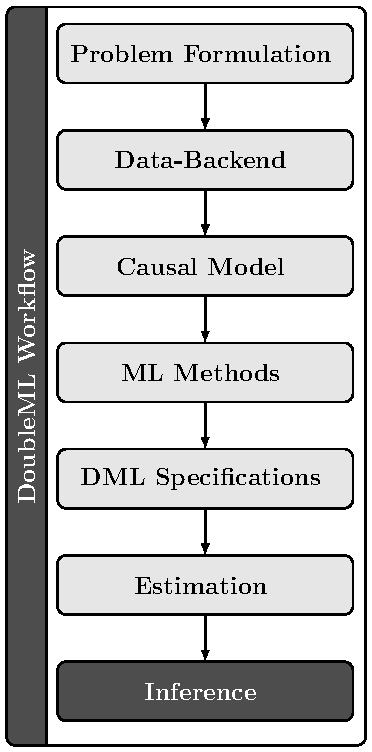
\includegraphics[width = \textwidth]{workflow/doubleml_workflow_inf.pdf}
\end{column}
\begin{column}{0.7\textwidth}
\begin{itemize}
\item Summary of the estimated effect
\end{itemize}
{\tiny
\begin{lstlisting}[language=Python,
backgroundcolor = \color{gray!20},
keywordstyle=\color{OliveGreen}, stringstyle=\color{BrickRed}]
dml_plr_forest$summary()
[1] "Estimates and significance testing of the effect of target variables"
     Estimate. Std. Error t value Pr(>|t|)    
e401      8969       1341   6.688 2.27e-11 ***
---
Signif. codes:  0 '***' 0.001 '**' 0.01 '*' 0.05 '.' 0.1 ' ' 1

\end{lstlisting}
}
\begin{itemize}
\item \textbf{Confidence interval(s)}
\end{itemize}
{\tiny
\begin{lstlisting}[language=Python,
backgroundcolor = \color{gray!20},
keywordstyle=\color{OliveGreen}, stringstyle=\color{BrickRed}]
dml_plr_forest$confint()
        2.5 %   97.5 %
e401 6340.356 11597.22
\end{lstlisting}
}
\begin{itemize}
\item \textbf{Multiplier bootstrap} \\
$\rightarrow$ relevant for multiple treatment effects!
\end{itemize}
{\tiny
\begin{lstlisting}[language=Python,
backgroundcolor = \color{gray!20},
keywordstyle=\color{OliveGreen}, stringstyle=\color{BrickRed}]
dml_plr_forest$bootstrap()
\end{lstlisting}
}
\begin{itemize}
\item Confidence interval(s) based on the multiplier bootstrap
\end{itemize}
{\tiny
\begin{lstlisting}[language=Python,
backgroundcolor = \color{gray!20},
keywordstyle=\color{OliveGreen}, stringstyle=\color{BrickRed}]
dml_plr_forest$confint(joint=TRUE)
        2.5 %   97.5 %
e401 6174.467 11763.11
\end{lstlisting}
}
\end{column}
\end{columns}
\end{frame}


%
%
%\begin{frame}[fragile]
%\frametitle{DoubleML API: R vs. Python}
%\begin{columns}
%\begin{column}{0.5\textwidth}
%\begin{block}{R}
%{\tiny
%\begin{lstlisting}[language=R, keywords={library},
%keywordstyle=\color{MidnightBlue}, stringstyle=\color{OliveGreen}]
%library(DoubleML)
%library(mlr3)
%library(mlr3learners)
%set.seed(1234)
%
%
%data_plr = make_plr_CCDDHNR2018(
%  alpha = 0.5, n_obs = 500, dim_x = 20,
%  return_type = 'data.table')
%obj_dml_data = DoubleMLData$new(
%  data_plr, y_col = 'y', d_cols = 'd')
%
%ml_g = lrn("regr.ranger")
%ml_m = lrn("regr.ranger")
%doubleml_plr = DoubleMLPLR$new(
%  obj_dml_data, ml_g, ml_m,
%  n_folds = 2, score = 'partialling out')
%
%doubleml_plr$fit()
%doubleml_plr$summary()
%   Estimate.  Std. Error  t value  Pr(>|t|)    
%d  0.51982    0.04061     12.8     <2e-16   ***
%\end{lstlisting}
%}
%\end{block}
%\end{column}
%\begin{column}{0.5\textwidth}
%\begin{block}{Python}
%{\tiny
%\begin{lstlisting}[language=Python,
%keywordstyle=\color{OliveGreen}, stringstyle=\color{BrickRed}]
%from doubleml import DoubleMLData, DoubleMLPLR
%from doubleml.datasets import make_plr_CCDDHNR2018
%import numpy as np
%from sklearn.ensemble import RandomForestRegressor
%np.random.seed(1234)
%
%data_plr = make_plr_CCDDHNR2018(
%    alpha = 0.5, n_obs = 500, dim_x = 20,
%    return_type = 'DataFrame')
%obj_dml_data = DoubleMLData(
%    data_plr, y_col = 'y', d_cols = 'd')
%
%ml_g = RandomForestRegressor()
%ml_m = RandomForestRegressor()
%doubleml_plr = DoubleMLPLR(
%    obj_dml_data, ml_g, ml_m,
%    n_folds = 2, score = 'partialling out')
%
%doubleml_plr.fit()
%doubleml_plr.summary
%  coef   std err t      P>|t| 2.5 % 97.5 %
% d 0.534 0.042   12.669 0.0   0.451 0.617
%\end{lstlisting}
%}
%\end{block}
%\end{column}
%\end{columns}
%
%\end{frame}
